\documentclass[tikz,border=12pt]{standalone}
\usepackage[T1]{fontenc}
\usepackage{lmodern}
\usetikzlibrary{positioning,arrows.meta,fit,backgrounds,shapes.geometric}
\definecolor{navy}{HTML}{09234F}\definecolor{blue}{HTML}{384CE3}\definecolor{sky}{HTML}{C4F0FF}
\definecolor{rule}{HTML}{CED3DC}\definecolor{paper}{HTML}{F6F8FB}\definecolor{ink}{HTML}{0B0F17}
\tikzset{
  box/.style={draw=navy,line width=.6pt,fill=white,rounded corners=2pt,align=center,font=\sffamily\small,minimum width=31mm,minimum height=11mm,text=ink},
  mod/.style={box,fill=sky!35},
  ext/.style={box,draw=blue,fill=blue!6},
  db/.style={cylinder,shape border rotate=90,aspect=.18,draw=navy,fill=white,align=center,font=\sffamily\small,minimum width=30mm,minimum height=14mm},
  grp/.style={draw=rule,fill=paper,rounded corners=4pt,inner sep=7pt},
  lab/.style={font=\sffamily\footnotesize\bfseries,text=navy,anchor=south west},
  arr/.style={-{Stealth[length=2.2mm]},draw=navy,line width=.55pt},
  store/.style={arr,dashed,draw=blue},
  note/.style={font=\sffamily\scriptsize,text=ink!70,fill=white,inner sep=1.5pt}
}
\begin{document}
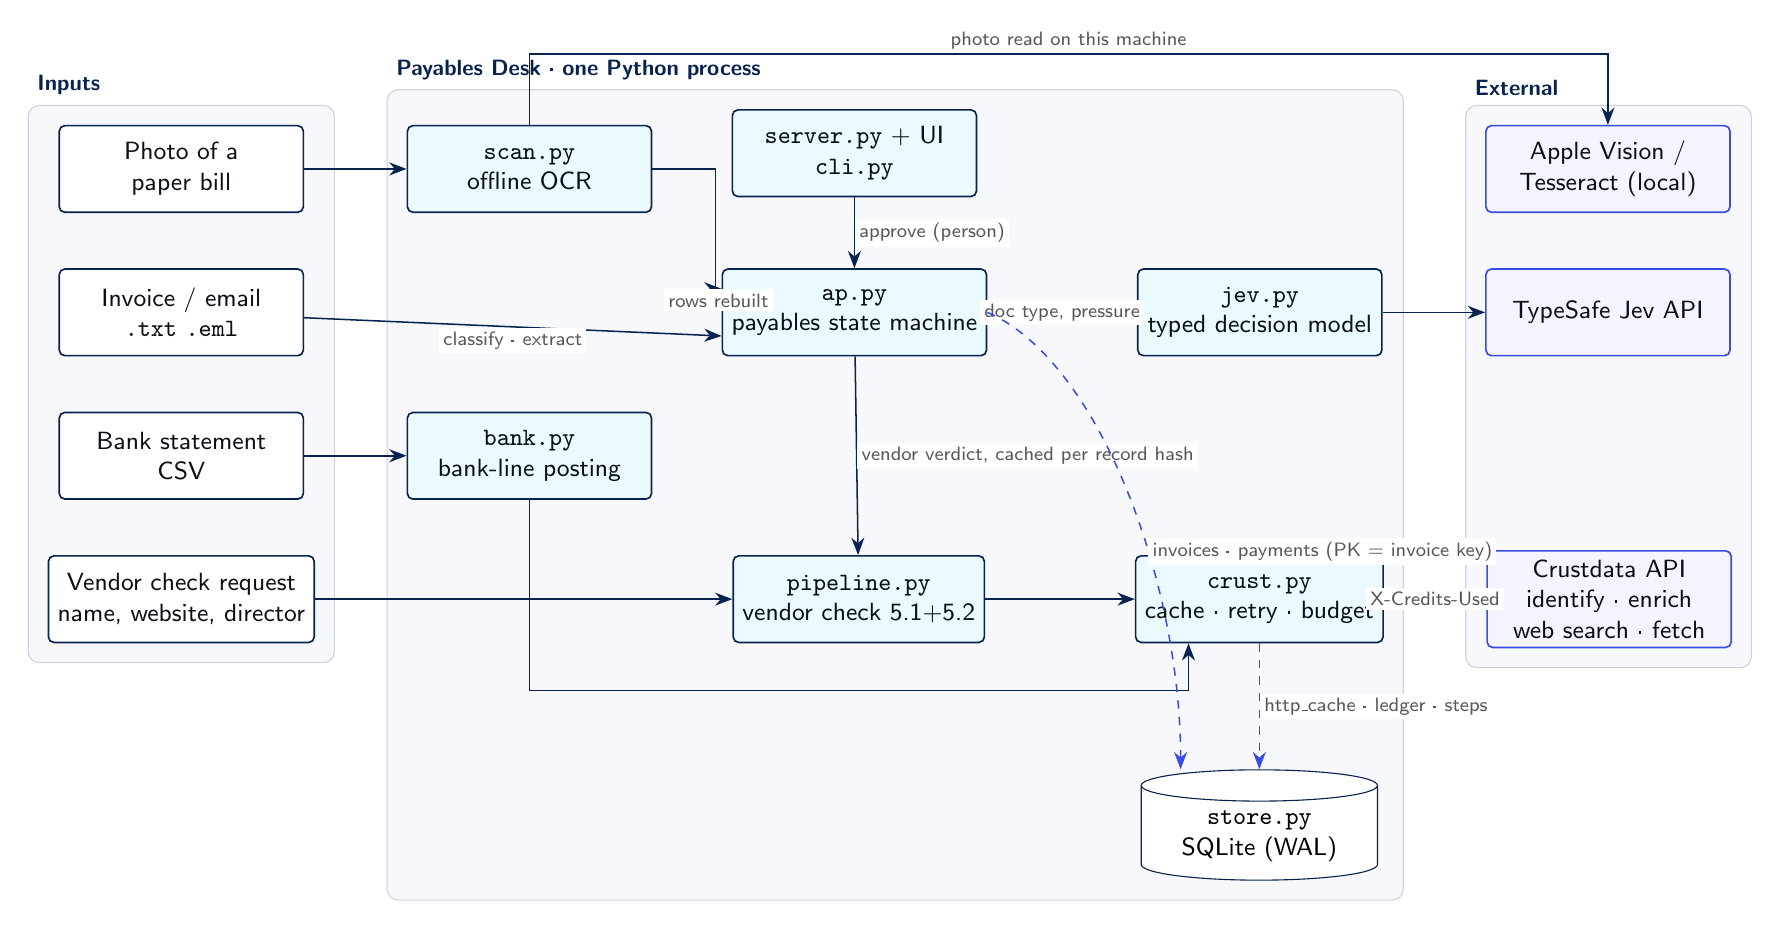
\begin{tikzpicture}[node distance=7mm and 13mm]
% inputs
\node[box] (photo) {Photo of a\\paper bill};
\node[box,below=of photo] (mail) {Invoice / email\\\texttt{.txt}\ \texttt{.eml}};
\node[box,below=of mail] (csv) {Bank statement\\CSV};
\node[box,below=of csv] (vreq) {Vendor check request\\name, website, director};
% modules
\node[mod,right=of photo] (scan) {\texttt{scan.py}\\offline OCR};
\node[mod,right=of mail,xshift=40mm] (ap) {\texttt{ap.py}\\payables state machine};
\node[mod,right=of csv] (bank) {\texttt{bank.py}\\bank-line posting};
\node[mod,right=of vreq,xshift=40mm] (pipe) {\texttt{pipeline.py}\\vendor check 5.1+5.2};
\node[mod,right=of ap,xshift=6mm] (jev) {\texttt{jev.py}\\typed decision model};
\node[mod,right=of pipe,xshift=6mm] (crust) {\texttt{crust.py}\\cache \textperiodcentered{} retry \textperiodcentered{} budget};
\node[db,below=16mm of crust] (store) {\texttt{store.py}\\SQLite (WAL)};
\node[mod,above=9mm of ap] (srv) {\texttt{server.py} + UI\\\texttt{cli.py}};
% externals
\node[ext,right=of jev] (ts) {TypeSafe Jev API};
\node[ext,right=of crust] (cd) {Crustdata API\\identify \textperiodcentered{} enrich\\web search \textperiodcentered{} fetch};
\node[ext,above=of ts] (ocr) {Apple Vision /\\Tesseract (local)};
% groups
\begin{scope}[on background layer]
\node[grp,fit=(photo)(vreq)] (gi) {};\node[lab] at (gi.north west) {Inputs};
\node[grp,fit=(scan)(bank)(ap)(pipe)(jev)(crust)(srv)(store)] (gd) {};\node[lab] at (gd.north west) {Payables Desk \textperiodcentered{} one Python process};
\node[grp,fit=(ocr)(ts)(cd)] (ge) {};\node[lab] at (ge.north west) {External};
\end{scope}
% flows
\draw[arr] (photo) -- (scan);
\draw[arr] (scan.east) -- ++(8mm,0) |- node[note,pos=.75,below]{rows rebuilt} ([yshift=3mm]ap.west);
\draw[arr] (mail) -- node[note,below]{classify \textperiodcentered{} extract} ([yshift=-3mm]ap.west);
\draw[arr] (csv) -- (bank);
\draw[arr] (vreq) -- (pipe);
\draw[arr] (srv) -- node[note,right]{approve (person)} (ap);
\draw[arr] (ap) -- node[note,right]{vendor verdict, cached per record hash} (pipe);
\draw[arr] (ap) -- node[note]{doc type, pressure} (jev);
\draw[arr] (pipe) -- (crust);
\draw[arr] (bank.south) |- ([yshift=-6mm]pipe.south) -| ([xshift=-9mm]crust.south);
\draw[arr] (crust) -- node[note]{X-Credits-Used} (cd);
\draw[arr] (jev) -- (ts);
\draw[arr] (scan.north) -- ++(0,9mm) -| node[note,pos=.25,above]{photo read on this machine} (ocr.north);
\draw[store] (crust.south) -- node[note,right]{http\_cache \textperiodcentered{} ledger \textperiodcentered{} steps} (store.north);
\draw[store] (ap.east) .. controls +(14mm,-6mm) and +(0mm,24mm) .. node[note,pos=.62,right]{invoices \textperiodcentered{} payments (PK = invoice key)} ([xshift=-10mm]store.north);
\end{tikzpicture}
\end{document}
